\section{Instructions: Language of the computer}
\subsection{Operations of the Computer Hardware}
\begin{frame}{Operations of the Computer Hardware}
\begin{figure}\caption{Arithmatic Instructions in MIPS}
\begin{center}
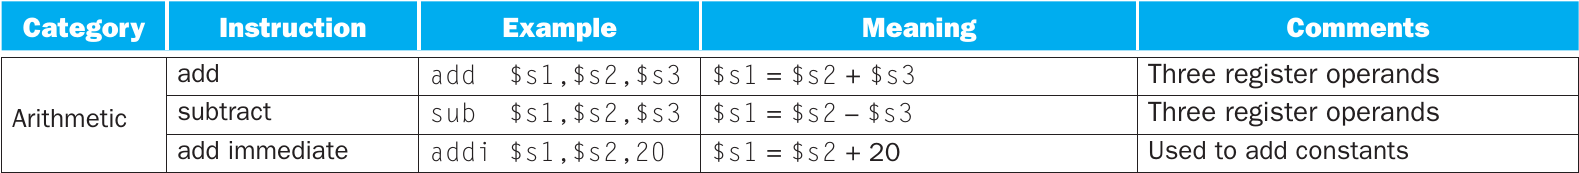
\includegraphics[width=\textwidth, height=0.2\textheight]{docs/images/operations-1}
\end{center}
\end{figure}
\end{frame}

\begin{frame}{Operations of the Computer Hardware (Cont'd)}
\begin{table}[H]
\begin{adjustbox}{width=\textwidth}
\begin{tabular}{|c|c|c|c|}
\hline
load word & \texttt{lw \$s1, 20(\$s2)} & \texttt{\$s1 = Memory[\$s2 + 20]} & Word from memory to register \\
\hline
store word & \texttt{sw \$s1, 20(\$s2)} & \texttt{Memory[\$s2 + 20] = \$s1} & Word from register to memory \\
\hline
load byte & \texttt{lb \$s1, 20(\$s2)} & \texttt{\$s1 = Memory[\$s2 + 20]} & Byte from memory to register \\
\hline
load byte unsigned & \texttt{lbu \$s1, 20(\$s2)} & \texttt{\$s1 = Memory[\$s2 + 20]} & Byte from memory to register \\
\hline
store byte & \texttt{sb \$s1, 20(\$s2)} & \texttt{Memory[\$s2 + 20] = \$s1} & Byte from register to memory \\
\hline
load upper immed & \texttt{lui \$s1, 20} & \texttt{\$s1 = 20 * $2^{16}$} & Loads constant in upper 16 bits \\
\hline
\end{tabular}
\end{adjustbox}
\caption{Data Transfer Instructions in MIPS}
\end{table}
\end{frame}

\begin{frame}{Operations of the Computer Hardware (Cont'd)}
\begin{figure}\caption{Logical Instructions in MIPS}
\begin{center}
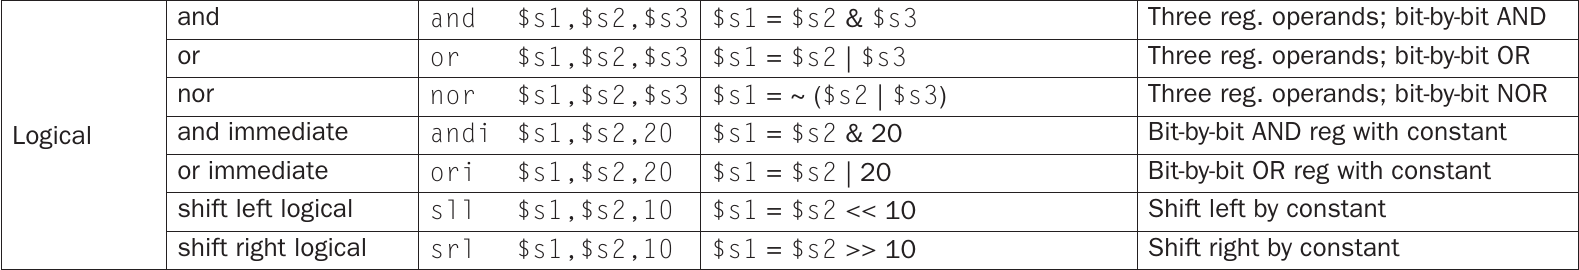
\includegraphics[width=\textwidth, height=0.4\textheight]{docs/images/operations-3}
\end{center}
\end{figure}
\end{frame}

\begin{frame}{Operations of the Computer Hardware (Cont'd)}
\begin{figure}\caption{Conditional Branch Instructions in MIPS}
\begin{center}
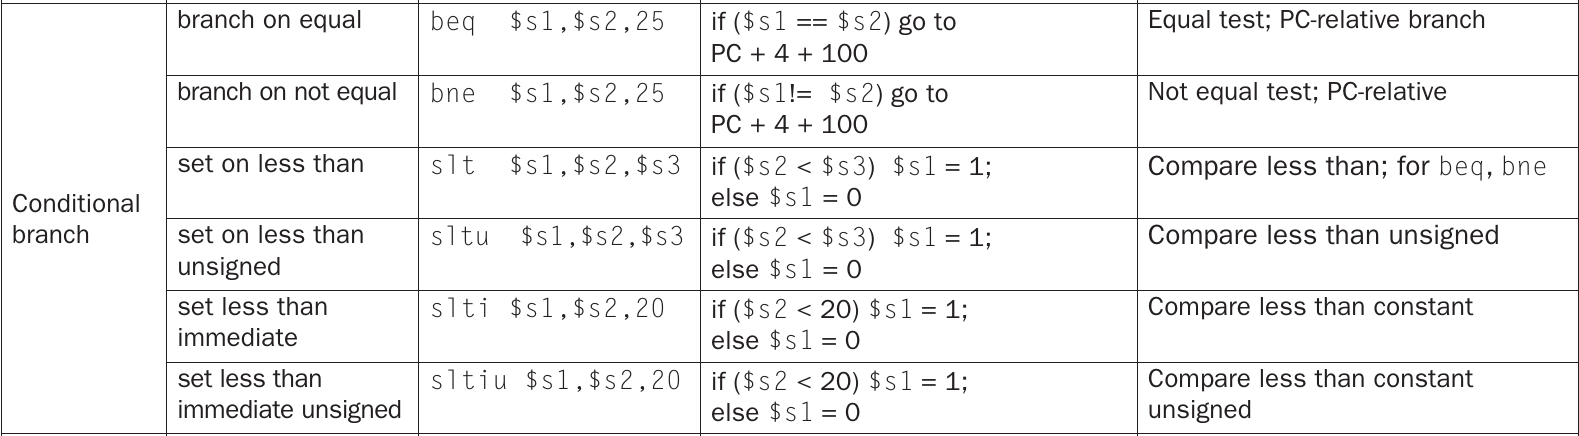
\includegraphics[width=\textwidth, height=0.5\textheight]{docs/images/operations-4}
\end{center}
\end{figure}
\end{frame}

\begin{frame}{Operations of the Computer Hardware (Cont'd)}
\begin{figure}\caption{Unconditional Jump Instructions in MIPS}
\begin{center}
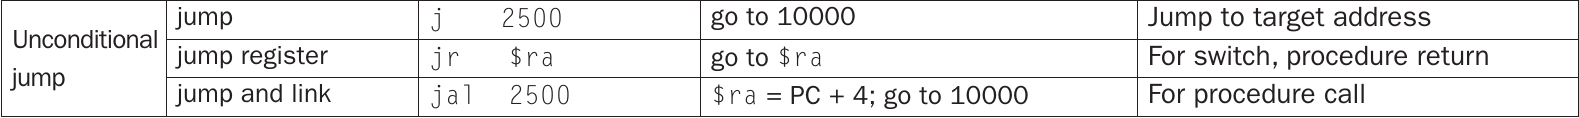
\includegraphics[width=\textwidth, height=0.17\textheight]{docs/images/operations-5  }
\end{center}
\end{figure}
\end{frame}

\subsection{Operands of the Computer Hardware}
\subsection{Representing Instructions}
\subsection{Logical Operations}
\subsection{Instuctions for Making Decisions}
\subsection{Suporting Precedures in Computer Hardware}
\subsection{MIPS Addressing for 32-Bit Immediates and Addresses}
\subsection{A C Sort Example to Put It All Together}